\def\lecturenumber{04}
\documentclass[11pt,a4paper]{article}
\usepackage[T1]{fontenc}
\usepackage[utf8]{inputenc}
\usepackage{lmodern}
\usepackage[margin=19mm,top=21mm,bottom=21mm,headheight=15pt]{geometry}
\usepackage{amsmath,amssymb,booktabs,array,graphicx,microtype}
\usepackage[dvipsnames]{xcolor}
\usepackage{enumitem,fancyhdr,listings,tcolorbox}
\usepackage[colorlinks=true,linkcolor=MidnightBlue,urlcolor=MidnightBlue]{hyperref}
\definecolor{courseblue}{HTML}{164B69}
\definecolor{pale}{HTML}{F0F5F7}
\pagestyle{fancy}
\fancyhf{}
\fancyhead[L]{\small\sffamily\color{courseblue}VALIDATED COMPUTING}
\fancyhead[R]{\small\sffamily Lecture \lecturenumber}
\fancyfoot[L]{\footnotesize Expanded lecture notes \textbullet\ October 2026}
\fancyfoot[R]{\footnotesize\thepage\ / 6}
\renewcommand{\headrulewidth}{0.4pt}
\setlength{\parindent}{0pt}
\setlength{\parskip}{5.5pt plus 1pt}
\setlength{\emergencystretch}{1.5em}
\setlist[itemize]{leftmargin=1.5em,itemsep=3pt,topsep=3pt}
\setlist[enumerate]{leftmargin=1.7em,itemsep=5pt,topsep=4pt}
\lstset{language=Python,basicstyle=\small\ttfamily,keywordstyle=\color{courseblue}\bfseries,
 commentstyle=\color{OliveGreen},stringstyle=\color{BrickRed},showstringspaces=false,
 columns=fullflexible,keepspaces=true,frame=single,rulecolor=\color{black!18},
 backgroundcolor=\color{black!2},aboveskip=6pt,belowskip=6pt,breaklines=true,
 xleftmargin=5pt,xrightmargin=5pt,framesep=5pt}
\newcommand{\R}{\mathbb R}
\newcommand{\fl}{\operatorname{fl}}
\newcommand{\abs}[1]{\left|#1\right|}
\newcommand{\heading}[2]{\section*{\color{courseblue}#1}\vspace{-4pt}{\small\sffamily\color{black!65}#2}\par\vspace{3pt}}
\newcommand{\opening}[2]{{\Large\sffamily\bfseries\color{courseblue}Lecture \lecturenumber\quad #1\par}\vspace{5pt}{\small #2}\par}
\newtcolorbox{question}[1]{colback=pale,colframe=courseblue!55,boxrule=0.4pt,
 arc=1mm,left=7pt,right=7pt,top=4pt,bottom=4pt,title={#1},fonttitle=\bfseries\small,
 coltitle=courseblue,colbacktitle=pale}
\newcommand{\reading}[1]{{\footnotesize\textbf{Reading and notebook.} #1\par}}
\hypersetup{pdfauthor={Validated Computing course},pdfsubject={Expanded introductory lecture notes with questions and exercises}}

\hypersetup{pdftitle={Lecture 04: Interval arithmetic as arithmetic with sets}}
\begin{document}
\opening{Interval arithmetic as arithmetic with sets}{Prerequisites: Lectures 01--03, inequalities and elementary functions.\newline
Goal: derive arithmetic rules that enclose every admissible input, before introducing rounding.}
\heading{1. Replace an unknown value by a set}{0--13 minutes: a measurement problem and the meaning of an enclosure}
Suppose a rectangle has length $l\in[2.9,3.1]$ metres and width
$w\in[4.8,5.2]$ metres. We want a statement valid for every allowed pair of
measurements, not just the area at their midpoints. Because both factors are
positive, the area satisfies
\[
 2.9\cdot4.8\le lw\le3.1\cdot5.2,
 \qquad lw\in[13.92,16.12]\ \text{square metres}.
\]
Both extrema occur among the allowed pairs if length and width may vary
independently. If an additional relation connects the measurements, the rectangle
of possible pairs may overstate the uncertainty. The same interval remains a
valid enclosure, but its extrema need not be physically attainable.

A closed bounded interval is the set
\[
 X=[a,b]=\{x\in\R:a\le x\le b\},\qquad a\le b.
\]
It is a \emph{point interval} when $a=b$. The brackets do not mean that the unknown
value is random, uniformly distributed, or probably close to the midpoint. They
state only which values are admitted. A probability model would be extra information.

\textbf{Two different uses of width.} An interval may describe uncertainty already
present in the data, or uncertainty in a numerical approximation to one exact
number. The first cannot be removed by increasing arithmetic precision. The
second may shrink with a better calculation. Later examples contain both sources
at once; a narrow printed interval is useful only if its meaning is clear.

Today the endpoints will be exact rationals. This separates the set argument from
machine rounding. In Python, describe intended decimals using strings:
\begin{lstlisting}
from fractions import Fraction
length = (Fraction("2.9"), Fraction("3.1"))
width = (Fraction("4.8"), Fraction("5.2"))
area = (length[0] * width[0], length[1] * width[1])
assert area == (Fraction("13.92"), Fraction("16.12"))
\end{lstlisting}
Here each pair stores lower and upper endpoints. It is not a new arithmetic type:
ordinary multiplication of Python tuples would not implement interval multiplication.
The formulas, and eventually a small class, supply the mathematical operations.

\begin{question}{Discuss the claim before computing}
The midpoint estimate is $3\cdot5=15$. Does the interval above prove that the area
is within one square metre of 15? If the area is actually fixed by a construction
constraint, what additional information would you need to obtain a smaller set?
\end{question}

\newpage
\heading{2. Interval geometry and set operations}{13--27 minutes: containment, intersections, and the information lost by a hull}
For $X=[a,b]$, define its width, midpoint, and radius by
\[
 w(X)=b-a,\qquad m(X)=\frac{a+b}{2},\qquad r(X)=\frac{b-a}{2}.
\]
Thus $X=[m-r,m+r]$ over the exact reals. These identities do not yet specify a
safe floating-point conversion: Lecture 05 will account for rounding the midpoint
and radius. A point interval has width zero; it is not empty.

Membership and containment are different comparisons. For $Y=[c,d]$,
\[
 x\in X\iff a\le x\le b,\qquad
 X\subseteq Y\iff c\le a\text{ and }b\le d.
\]
A statement about an entire interval must check both endpoints. Testing whether
its midpoint lies in another interval is insufficient.

The smallest interval containing both $X$ and $Y$ is their \emph{hull}:
\[
 \operatorname{hull}(X,Y)=[\min(a,c),\max(b,d)].
\]
Their intersection is $[\max(a,c),\min(b,d)]$ if the proposed endpoints are
ordered; otherwise it is empty. For $X=[0,1]$ and $Y=[2,3]$, the intersection
is empty, the union has a gap, and the hull is $[0,3]$.
\begin{center}
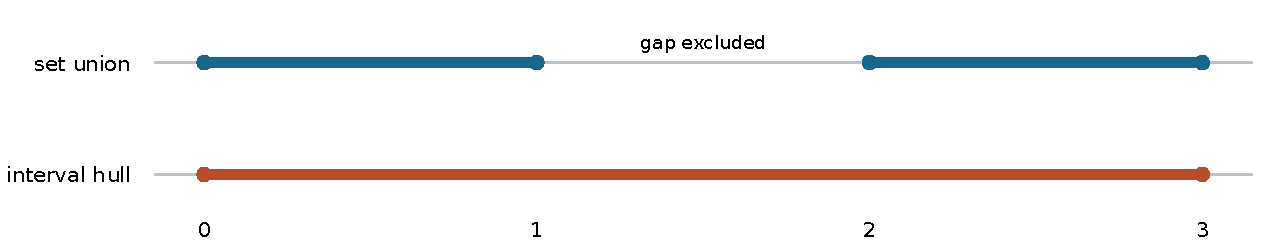
\includegraphics[width=0.9\linewidth]{figures/interval_union_hull.pdf}
\end{center}
The hull forgets the gap. That makes it convenient to store with two endpoints,
but unsuitable for a claim that every point in the hull is attainable.
In contrast, $[0,1]\cap[1,2]=\{1\}$: touching intervals have a nonempty intersection.

\textbf{A useful consistency check.} If two intervals independently enclose the
\emph{same} exact quantity, their intersection also encloses it. An empty
intersection means that at least one purported guarantee or input interpretation
is wrong. Intersecting intervals for two unrelated quantities has no such meaning.

\begin{question}{Draw before answering}
For $X=[-2,1]$ and $Y=[0,3]$, find the intersection, hull, widths, and midpoints.
Is $X\subseteq Y$? Can a proper subset have the same midpoint as the larger interval?
Give an example and explain why midpoint comparison cannot decide containment.
\end{question}

\newpage
\heading{3. Derive arithmetic from independent choices}{27--45 minutes: endpoint proofs and a readable multiplication rule}
For a real operation $\circ$ defined on every input pair, its set extension is
\[
 X\circ Y=\{x\circ y:x\in X,\ y\in Y\}.
\]
The two choices are independent. For $X=[a,b]$ and $Y=[c,d]$, addition,
negation, and subtraction give
\[
 X+Y=[a+c,b+d],\quad -X=[-b,-a],\quad X-Y=[a-d,b-c].
\]
For subtraction, $x\ge a$ and $y\le d$ imply $x-y\ge a-d$; the opposite
inequalities give $x-y\le b-c$. Both bounds are attained. Varying the inputs
continuously fills the values between them. For example,
$[1,4]-[2,5]=[-4,2]$, not $[-1,-1]$.

\textbf{Multiplication requires four corners.} The correct general formula is
\[
 XY=[\min(ac,ad,bc,bd),\max(ac,ad,bc,bd)].
\]
For fixed $y$, the product is linear in $x$, so an extremum occurs at an endpoint.
Apply the same argument to $y$ for each endpoint of $X$. This proves that the
extrema occur at the corners. Since the rectangle of inputs is connected and
multiplication is continuous, its image contains the intermediate values too.

Take $X=[-2,3]$ and $Y=[-4,-1]$. The corner products are $8,2,-12,-3$,
so the exact set product is $[-12,8]$. The shortcut $[ac,bd]=[8,-3]$ fails:
it ignored how multiplication reverses inequalities when a factor is negative.
\begin{lstlisting}
def multiply_intervals(X, Y):
    a, b = X
    c, d = Y
    products = [a*c, a*d, b*c, b*d]
    lower = min(products)
    upper = max(products)
    return lower, upper

X = (Fraction(-2), Fraction(3))
Y = (Fraction(-4), Fraction(-1))
assert multiply_intervals(X, Y) == (Fraction(-12), Fraction(8))
\end{lstlisting}
All inputs here are ordered pairs of rational endpoints. Consequently the four
products and the endpoint comparisons are exact. This short function deliberately
exposes the full rule; sign-based optimizations can wait until the proof is familiar.

\begin{question}{Find the extremizing input pairs}
For $[-3,-1][2,5]$, identify the lower and upper products and the input pair
attaining each. Repeat for $[-1,2][-2,4]$. Why can testing only the two interval
midpoints miss both extrema? What changes when one factor is a point interval?
\end{question}

\newpage
\heading{4. Division requires a domain check}{45--59 minutes: negative reciprocals and the obstruction at zero}
If $0\notin Y=[c,d]$, the function $y\mapsto1/y$ is continuous and strictly
decreasing on $Y$. Hence
\[
 \frac1Y=[1/d,1/c],\qquad \frac XY=X\left(\frac1Y\right).
\]
This is valid for a wholly negative interval as well as a positive one.
For example, $1/[-4,-2]=[-1/2,-1/4]$, and
$[1,2]/[-4,-2]=[-1,-1/4]$. Reversing the reciprocal endpoints correctly is
more important than remembering a separate rule for every sign pattern.
\begin{lstlisting}
def reciprocal_interval(Y):
    lower, upper = Y
    if lower <= 0 <= upper:
        raise ZeroDivisionError("Denominator interval includes zero")
    return Fraction(1) / upper, Fraction(1) / lower

Y = (Fraction(-4), Fraction(-2))
assert reciprocal_interval(Y) == (Fraction(-1, 2), Fraction(-1, 4))
\end{lstlisting}
The use of \texttt{Fraction(1)} makes the intended rational arithmetic explicit.
Dividing ordinary Python integers using \texttt{/} would instead produce floats.
Scalar data can be viewed as point intervals, but their representation still matters.

\textbf{Why reject an interval containing zero?} On $[-1,1]$, reciprocals of
the nonzero points form
\[
 (-\infty,-1]\ \cup\ [1,\infty).
\]
No bounded interval encloses this set. Moreover, the expression is undefined at
zero itself. Even $[0,1]$ causes unbounded reciprocals near zero. Our elementary
arithmetic requires the operation to be defined for every admissible input, and
uses only bounded intervals. It therefore rejects all these divisions explicitly.
A zero numerator does not make the excluded case $0/0$ a valid operation.

This is a scope decision, not a claim that every possible interval library must
stop in the same way. Richer representations may keep unbounded intervals or
unions and attach domain information. Quietly returning a convenient bounded
answer would not implement those richer semantics.

\begin{question}{Can algebra repair the domain?}
The expressions $x/x$ and $1$ agree for $x\ne0$. May we replace the first by the
second while claiming to evaluate it everywhere on $[-1,1]$? What if the declared
domain is $[1,2]$? Distinguish an algebraic identity on its domain from an extension
to points at which the original expression was undefined.
\end{question}

\newpage
\heading{5. Composition preserves inclusion, not dependence}{59--75 minutes: square, repeated variables, and a general proof}
For one unknown $x\in X=[-2,3]$, the expression $x^2$ uses the same value twice.
The two-operand set product $XX$ permits two independent values and gives
$[-6,9]$. It is an enclosure of every square, but the exact square range is $[0,9]$.
The impossible negative values come from pairs such as $(-2,3)$, not from rounding.

A dedicated square operation retains the one-variable relation:
\[
 \operatorname{square}([a,b])=
 \begin{cases}
 [a^2,b^2], & 0\le a,\\
 [b^2,a^2], & b\le0,\\
 [0,\max(a^2,b^2)], & a<0<b.
 \end{cases}
\]
On each side of zero use monotonicity; if zero belongs to the interval, zero is
an attainable minimum. Similarly $X-X=[a-b,b-a]$, whereas the range of $x-x$
is the singleton $\{0\}$. Naming both operands \texttt{X} does not force an interval
arithmetic operation to remember that their values must coincide.

\textbf{Composition theorem.} Suppose every elementary operation returns a set
containing its exact result for all allowed operands, and all operations are
defined on their intermediate input sets. Then a finite expression built from
these operations encloses its exact value for every admissible original input.

To prove this, fix one original input. Its value belongs to its input interval.
At the first operation, the enclosure property puts the exact intermediate result
in the computed set. Repeat along the expression's evaluation order. The final
set contains the exact answer. Since the original input was arbitrary, the claim
holds for the entire domain. This proof does not say that all combinations allowed
at later operations can arise from one original input.

\textbf{A complete simple conclusion.} For $X=[2,3]$,
\[
 X+1/X=[2,3]+[1/3,1/2]=[7/3,7/2].
\]
Thus $x+1/x>0$ for every $x\in[2,3]$. We have proved positivity without finding
the exact minimum. A non-sharp interval can be entirely sufficient for the claim.

\textbf{Ordinary algebra needs care.} In exact interval arithmetic,
$X(Y+Z)\subseteq XY+XZ$, but equality can fail: the right side permits different
values of $x$ in its two products. With $X=[-1,1]$, $Y=[1,1]$, and $Z=[-1,-1]$,
the left side is $[0,0]$ and the right side is $[-2,2]$. Interval arithmetic
retains inclusion while giving up some familiar field identities.

\newpage
\heading{6. Exercises and an implementation contract}{75--90 minutes: check one proof and one implementation in pairs}
Our rational teaching functions assume ordered, finite endpoint pairs and exact
rational operations. A small class should enforce these assumptions at construction,
represent an empty intersection explicitly, and reject unsupported divisions.
Test cases can reveal mistakes; the endpoint proofs establish the all-input guarantee.
\begin{enumerate}
\item \textbf{Compute and justify.} For $X=[-3,2]$ and $Y=[-2,4]$, compute
$X+Y$, $X-Y$, $XY$, the hull, and the intersection. Identify inputs attaining the
product extrema. Explain why the midpoint product is not a bound.
\item \textbf{Retain one occurrence.} Implement a square-range function with
rational endpoints. Check intervals entirely positive, entirely negative, crossing
zero, and consisting of the single point zero. Compare it with multiplication of
an interval by itself. State a condition under which these operations agree.
\item \textbf{Intersect only comparable claims.} Two programs claim enclosures
$[1,2]$ and $[3/2,5/2]$ for the same exact quantity. What improved enclosure follows?
What if the second interval were $[3,4]$? Why would the conclusion change if the
two intervals described different physical measurements?
\item \textbf{A valid but non-sharp range.} Check the enclosure for $x+1/x$ on
$[2,3]$ from page 5. Then use $f'(x)=1-1/x^2$ to find the exact range. Which
information did the interval addition forget? Why does the wider range still
prove the positivity claim?
\item \textbf{Prove inclusion isotonicity.} If $X\subseteq X'$ and $Y\subseteq Y'$,
show that $X+Y\subseteq X'+Y'$ and $XY\subseteq X'Y'$. Use the definition by
independent choices rather than splitting into many sign cases. For division,
state the additional domain assumption needed on $Y'$.
\end{enumerate}
\begin{question}{Before approving a result}
What exact input set was intended? Were the endpoints represented exactly? Is each
operation defined on all admitted intermediate values? Does the final set prove
the requested claim, or merely fail to refute it? Locate each premise in one of
your exercise solutions.
\end{question}
\textbf{Selected checks.} Exercise 1 gives $[-5,6]$, $[-7,4]$, $[-12,8]$,
hull $[-3,4]$, and intersection $[-2,2]$. In Exercise 2, agreement holds when the
interval has one sign, including an endpoint at zero. Exercise 3 gives $[3/2,2]$;
an empty intersection would expose inconsistent guarantees for the same quantity.
The exact range in Exercise 4 is $[5/2,10/3]$.

\reading{Companion: \texttt{notebooks/04\_interval\_basics.ipynb}; Lab 04: build a rational
interval class. Tucker, \emph{Validated Numerics} (2011), \S\S2.1--2.2, pp. 24--30.
The notebook's \texttt{vc.intervals} package implements these rules; the excerpts
here use only Python's standard library. Next: preserving inclusion with machine endpoints.}
\end{document}
